\documentclass[12pt,a4paper]{article}

\usepackage[utf8]{inputenc}
\usepackage[T1]{fontenc}
\usepackage[french]{babel}
\usepackage{lmodern}
\usepackage{geometry}
\usepackage{graphicx}
\usepackage{booktabs}
\usepackage{float}
\usepackage{amsmath}
\usepackage{hyperref}

\geometry{margin=2.5cm}
\graphicspath{{../figures/}}

\begin{document}

% --- DÉBUT DE LA PAGE DE GARDE ---
\begin{titlepage}
    \centering
    \vspace*{1cm}

    % Logo INSEA (Assurez-vous d'avoir un fichier insea_logo.png/jpg dans votre dossier figures)
    
\includegraphics[width=0.4\textwidth]{../INSEA_logo.png} \par
    \vspace{2.5cm}

    % Module et Professeur
    {\Large \textbf{Module : Séries Chronologiques}}\par
    \vspace{0.5cm}
    {\large Encadré par : Mme Badaoui}\par
    \vspace{2.5cm}

    % Titre du projet
    {\huge \textbf{Application de la méthode de Box-Jenkins}}\par
    \vspace{0.5cm}
    {\Large \textit{Prévision des ventes mensuelles de voitures au Québec}}\par
    \vspace{3cm}

    % Auteur
    {\large Réalisé par :}\par
    \vspace{0.5cm}
    \textbf{\Huge \scshape Ait Bargach Ahmed}\par

    \vfill

    % Année universitaire (en bas de page)
    {\large Année universitaire 2025--2026}\par
\end{titlepage}



\begin{abstract}
Ce rapport applique la méthodologie de Box-Jenkins à une série mensuelle de ventes
de voitures au Québec, observée de janvier 1960 à décembre 1968. L'objectif est de
construire un modèle de prévision simple, interprétable et validé sur un échantillon
test. La série présente une tendance croissante et une saisonnalité annuelle nette.
Après transformation logarithmique et différenciations ordinaire et saisonnière, un
modèle SARIMA est estimé. Le modèle retenu, SARIMA$(3,1,1)(0,1,0)_{12}$, donne une
erreur moyenne absolue d'environ 160 ventes sur la période de validation, soit un
MAPE proche de 0,73 \%.
\end{abstract}

\section{Introduction}

Une série chronologique est une suite d'observations ordonnées dans le temps.
L'objectif principal du travail demandé est d'appliquer la méthode de Box et Jenkins :
visualiser la série, étudier sa tendance et sa saisonnalité, la rendre stationnaire,
identifier un modèle à partir des corrélogrammes, estimer ce modèle, valider les
résidus puis produire des prévisions.

La démarche suivie reprend les étapes vues dans le cours : description des données,
décomposition tendance/saisonnalité, tests de stationnarité, analyse des fonctions
d'autocorrélation ACF et PACF, estimation SARIMA, validation et prévision finale.

\section{Description des données}

La série utilisée contient les ventes mensuelles de voitures au Québec entre janvier
1960 et décembre 1968. Elle contient donc 108 observations mensuelles. La variable
étudiée est le nombre de ventes par mois.

\begin{table}[H]
\centering
\begin{tabular}{lr}
\toprule
Statistique & Valeur \\
\midrule
Nombre d'observations & 108 \\
Minimum & 6 550 \\
Premier quartile & 11 300 \\
Médiane & 14 493,5 \\
Moyenne & 15 396,0 \\
Troisième quartile & 18 152 \\
Maximum & 29 500 \\
\bottomrule
\end{tabular}
\caption{Statistiques descriptives de la série.}
\end{table}

La figure \ref{fig:serie} montre une croissance globale des ventes au cours du temps.
On observe aussi une répétition annuelle : les ventes sont généralement plus élevées
au printemps et plus faibles au début ou à la fin de certaines années. Cela justifie
l'utilisation d'un modèle saisonnier de période $s=12$.

\begin{figure}[H]
\centering
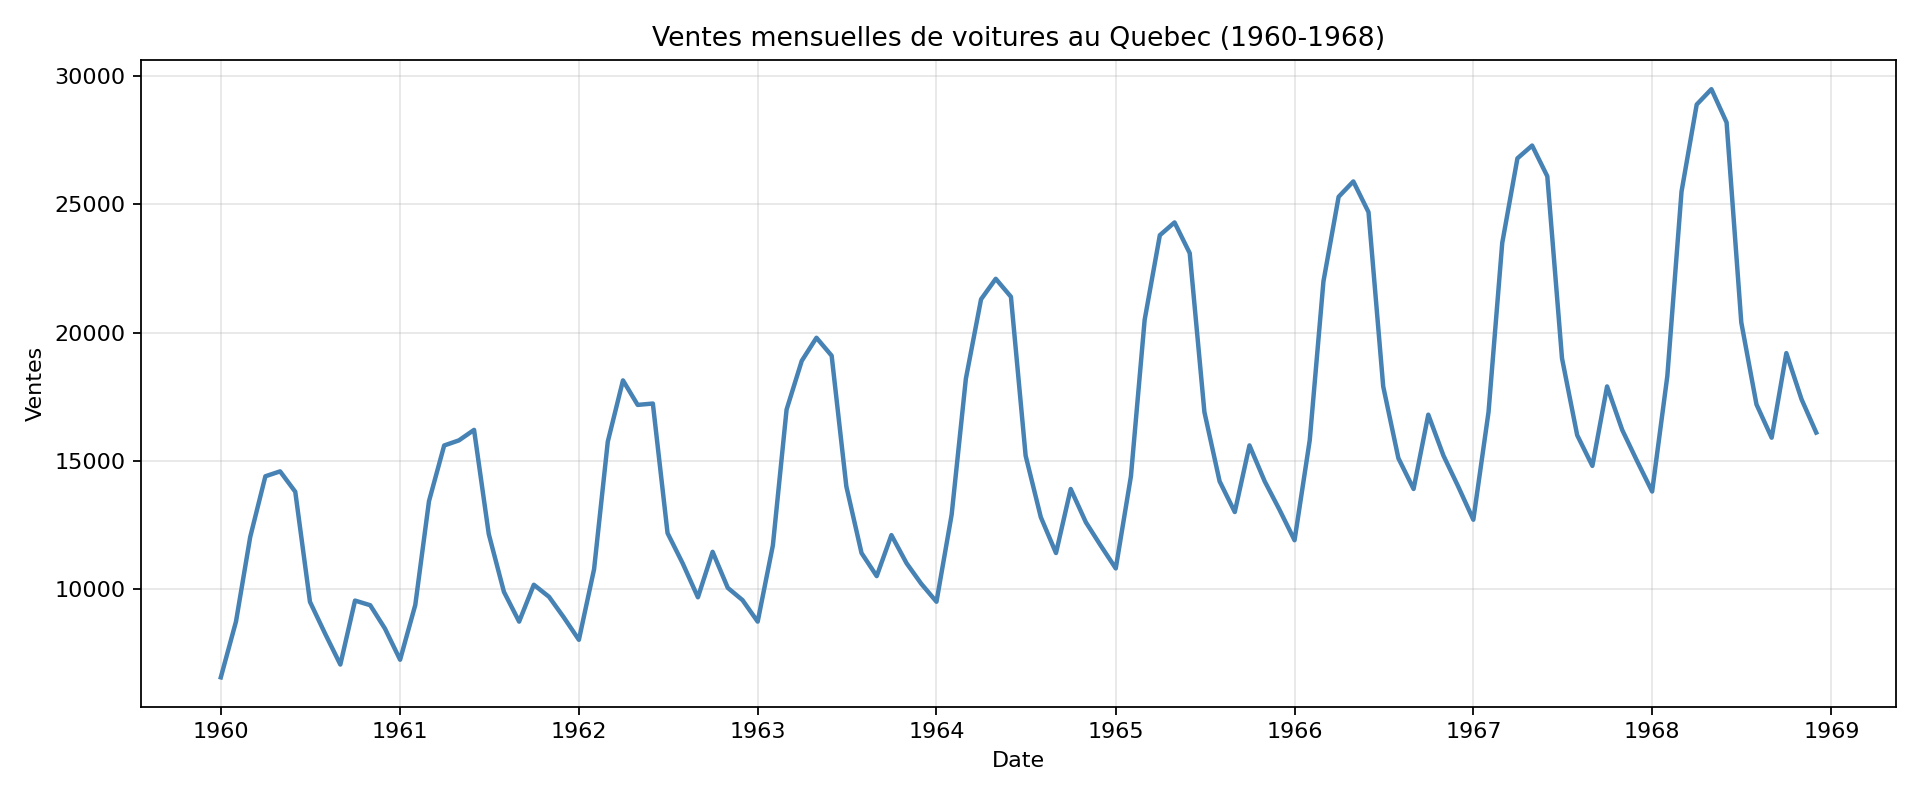
\includegraphics[width=0.92\textwidth]{serie_complete.png}
\caption{Série complète des ventes mensuelles.}
\label{fig:serie}
\end{figure}

\section{Échantillons d'apprentissage et de validation}

Conformément à l'énoncé, les données sont divisées en deux parties. Le modèle est
estimé sur la période janvier 1960 -- décembre 1966, puis évalué sur janvier 1967 --
décembre 1968.

\begin{table}[H]
\centering
\begin{tabular}{lcc}
\toprule
Échantillon & Période & Taille \\
\midrule
Apprentissage & 1960-01 à 1966-12 & 84 \\
Validation & 1967-01 à 1968-12 & 24 \\
\bottomrule
\end{tabular}
\caption{Découpage des données.}
\end{table}

\begin{figure}[H]
\centering
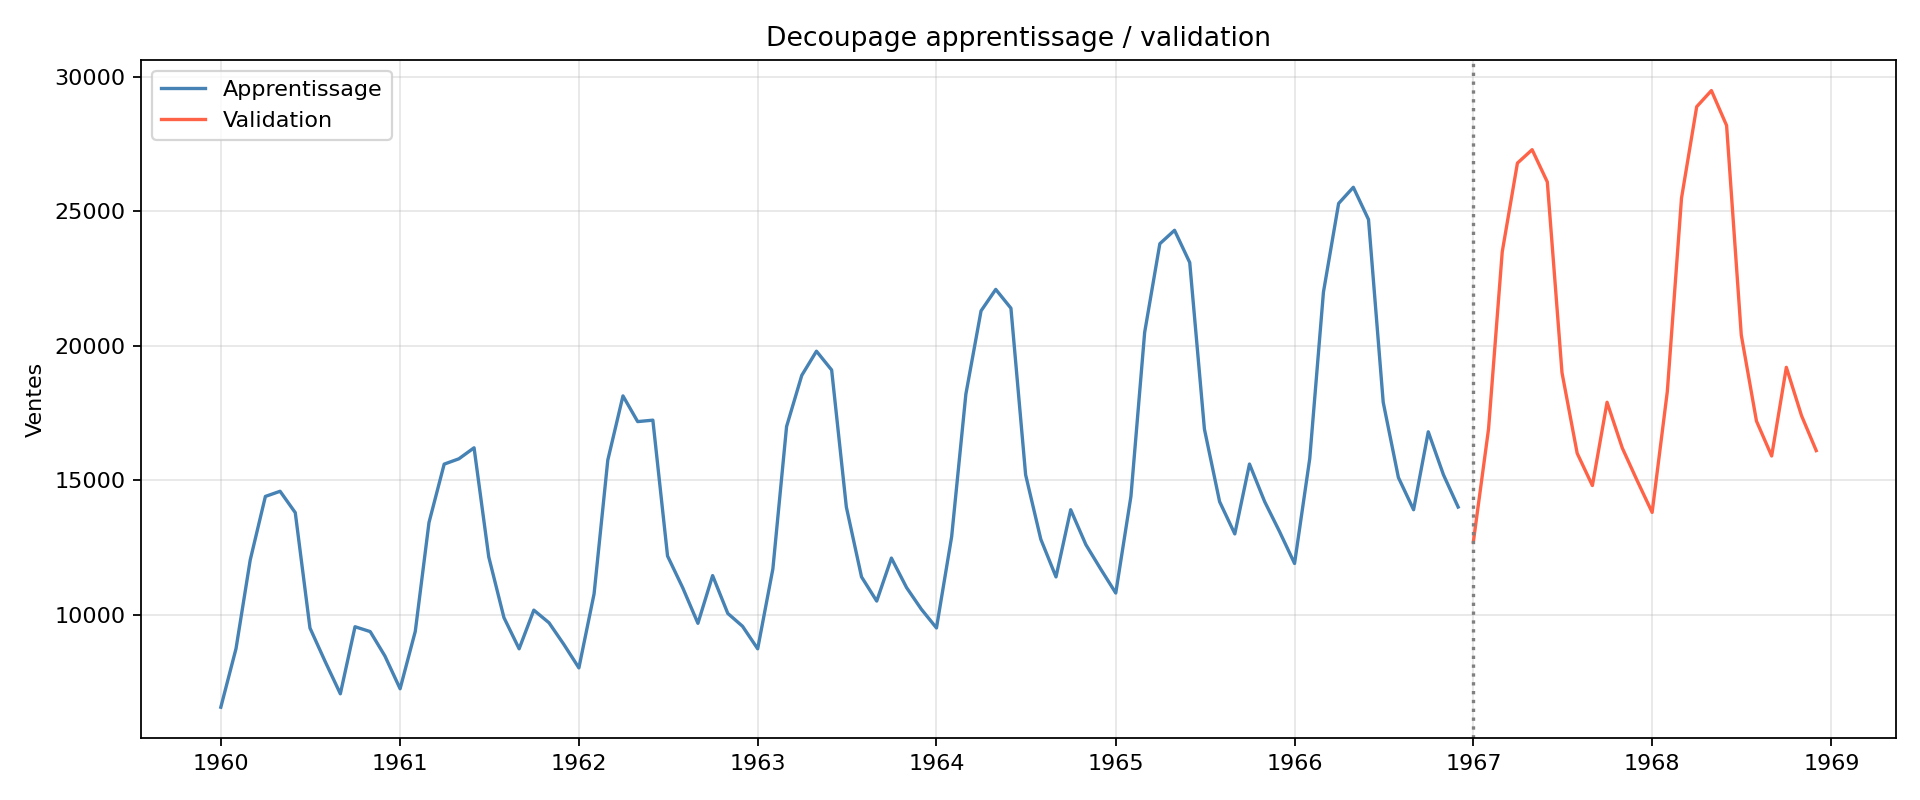
\includegraphics[width=0.92\textwidth]{split_train_test.png}
\caption{Séparation apprentissage / validation.}
\end{figure}

\section{Analyse qualitative}

La série présente deux composantes importantes :
\begin{itemize}
    \item une tendance croissante : le niveau moyen des ventes augmente entre 1960 et 1968 ;
    \item une saisonnalité annuelle : certains mois reviennent régulièrement avec des niveaux plus élevés.
\end{itemize}

\begin{figure}[H]
\centering
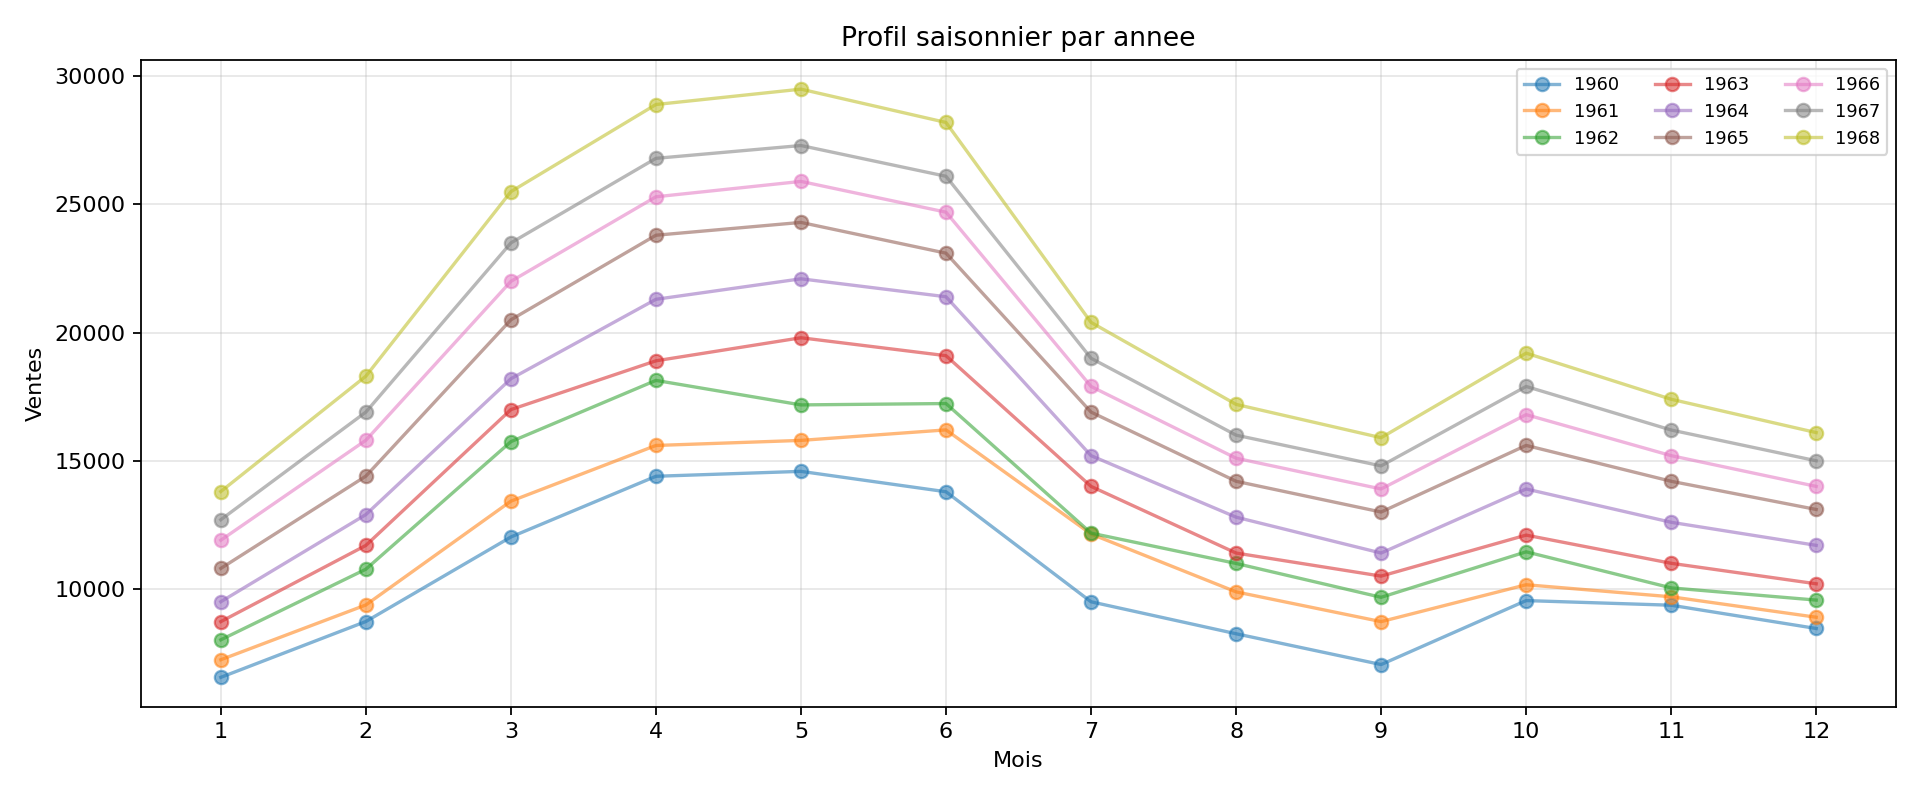
\includegraphics[width=0.92\textwidth]{saisonnalite.png}
\caption{Profil saisonnier des ventes par année.}
\end{figure}

La décomposition multiplicative est adaptée car l'amplitude saisonnière augmente avec
le niveau de la série. On peut écrire, de manière simplifiée :
\[
Y_t = T_t \times S_t \times R_t,
\]
où $T_t$ est la tendance, $S_t$ la composante saisonnière et $R_t$ le résidu.

\begin{figure}[H]
\centering
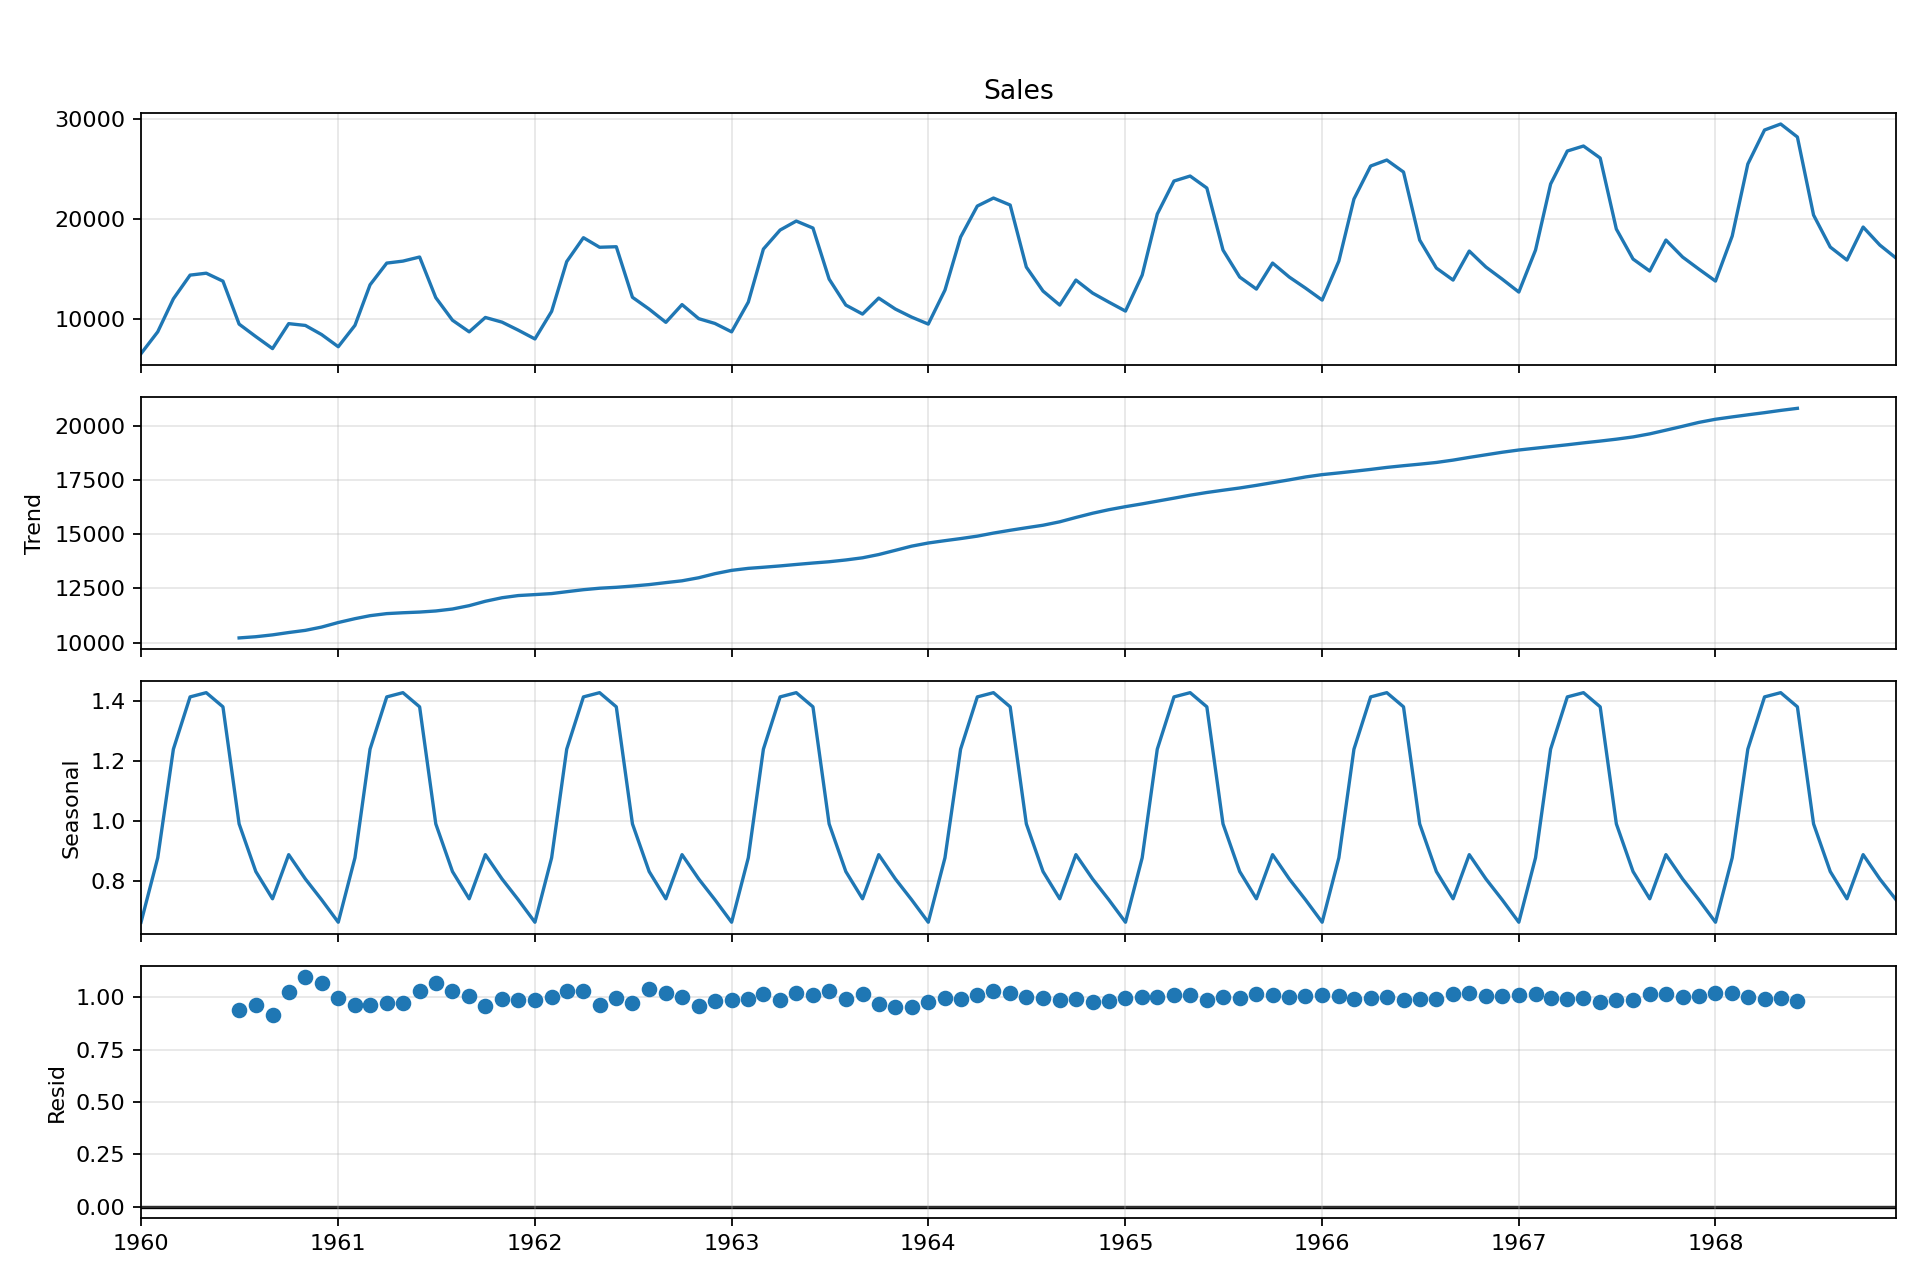
\includegraphics[width=0.92\textwidth]{decomposition.png}
\caption{Décomposition multiplicative de la série.}
\end{figure}

\section{Stationnarité}

La méthode de Box-Jenkins suppose de travailler sur une série stationnaire. La série
brute n'est pas stationnaire : le test ADF ne rejette pas la racine unitaire et le test
KPSS rejette l'hypothèse de stationnarité. Comme la saisonnalité semble multiplicative,
on applique d'abord une transformation logarithmique. Ensuite, on utilise une
différenciation ordinaire et une différenciation saisonnière :
\[
Z_t = (1-B)(1-B^{12})\log(Y_t).
\]

\begin{table}[H]
\centering
\begin{tabular}{lcc}
\toprule
Série testée & p-value ADF & p-value KPSS \\
\midrule
Série brute & 0,9886 & 0,0100 \\
$\log(Y_t)$ & 0,7168 & 0,0100 \\
$\Delta \log(Y_t)$ & 0,0002 & 0,1000 \\
$\Delta \Delta_{12} \log(Y_t)$ & 0,0089 & 0,1000 \\
\bottomrule
\end{tabular}
\caption{Tests de stationnarité sur l'échantillon d'apprentissage.}
\end{table}

Après transformation et différenciations, la série devient stationnaire : la p-value du
test ADF est inférieure à 5 \% et celle du test KPSS est supérieure à 5 \%.

\begin{figure}[H]
\centering
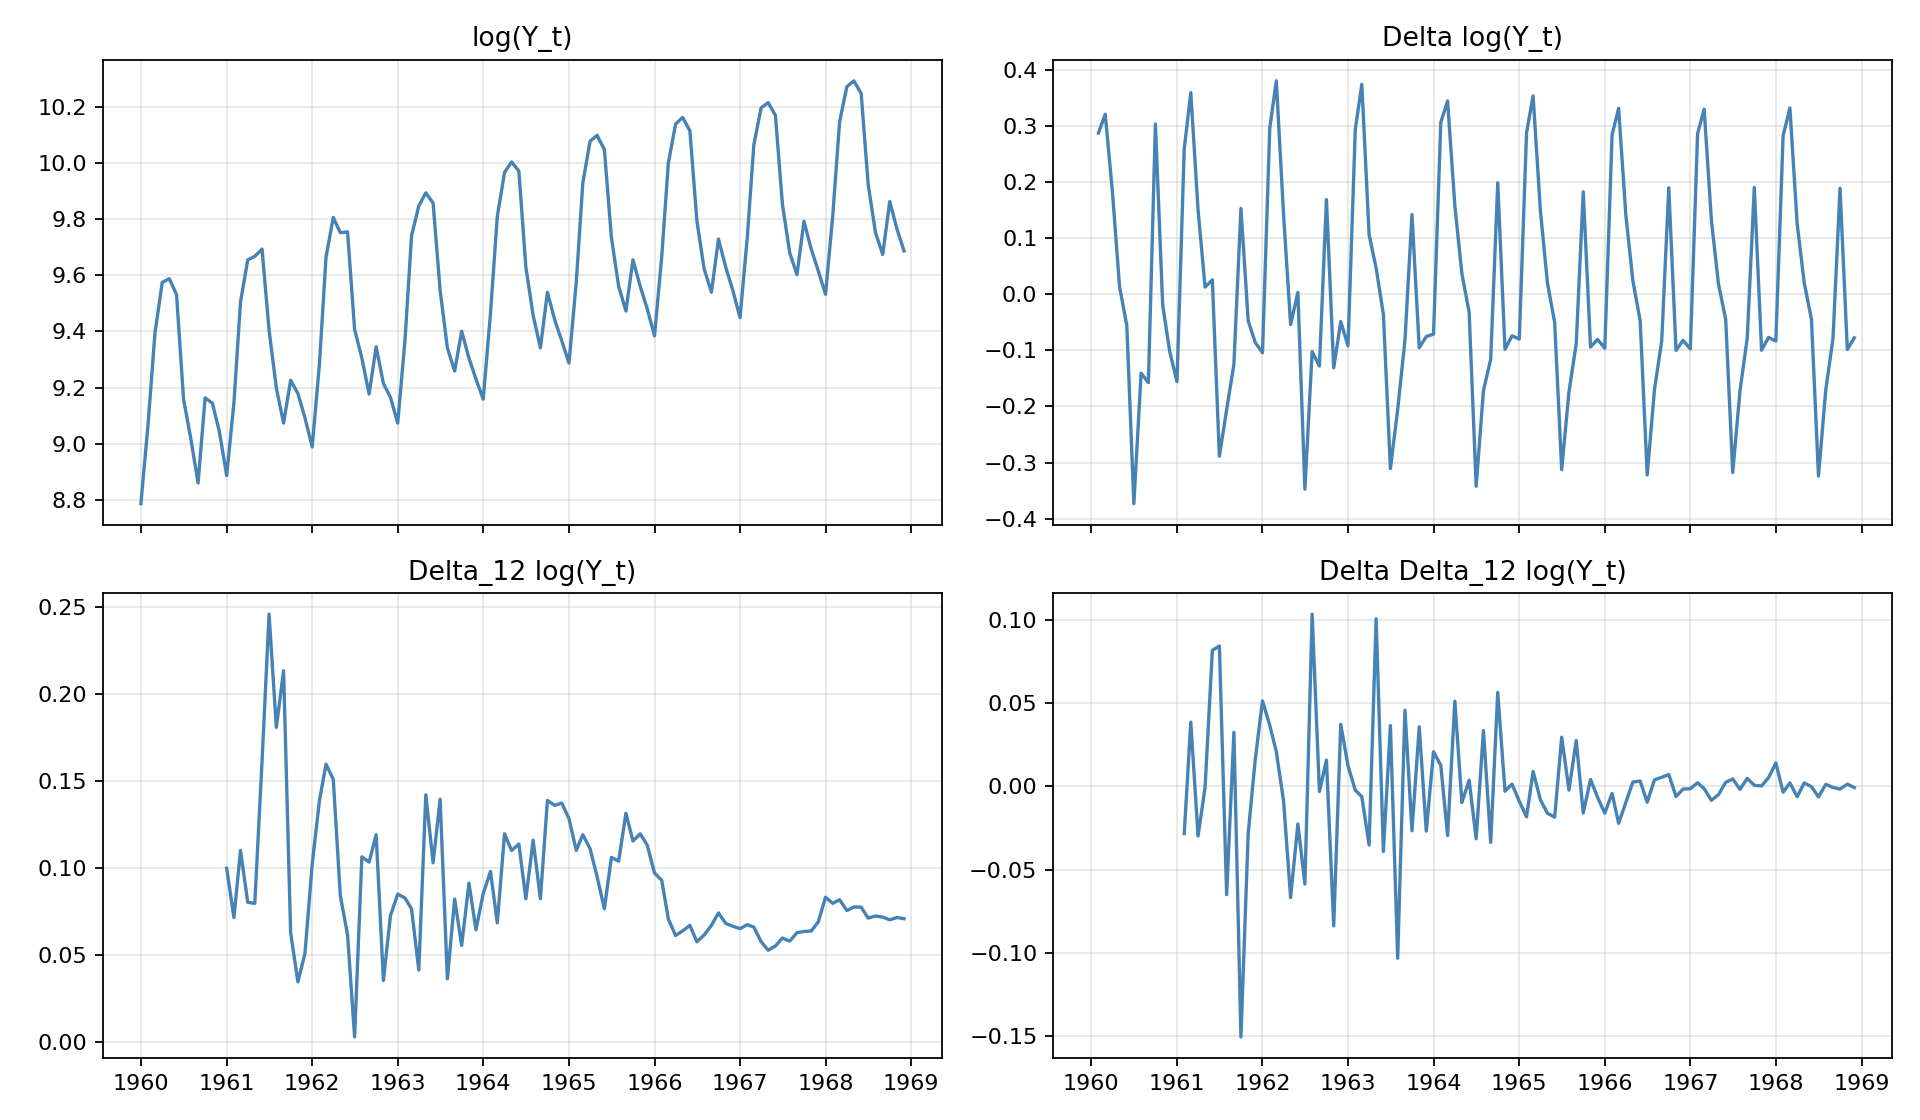
\includegraphics[width=0.92\textwidth]{transformations.png}
\caption{Transformations utilisées pour stabiliser la série.}
\end{figure}

\section{Corrélogrammes ACF et PACF}

Les corrélogrammes ACF et PACF sont tracés jusqu'au retard $K=36$, comme demandé dans
l'énoncé. Après différenciation, les autocorrélations deviennent rapidement plus faibles,
ce qui confirme que la série transformée est exploitable dans un modèle ARMA/SARIMA.
Les premiers retards restent informatifs, ce qui motive la recherche sur de petits
ordres $p$ et $q$.

\begin{figure}[H]
\centering
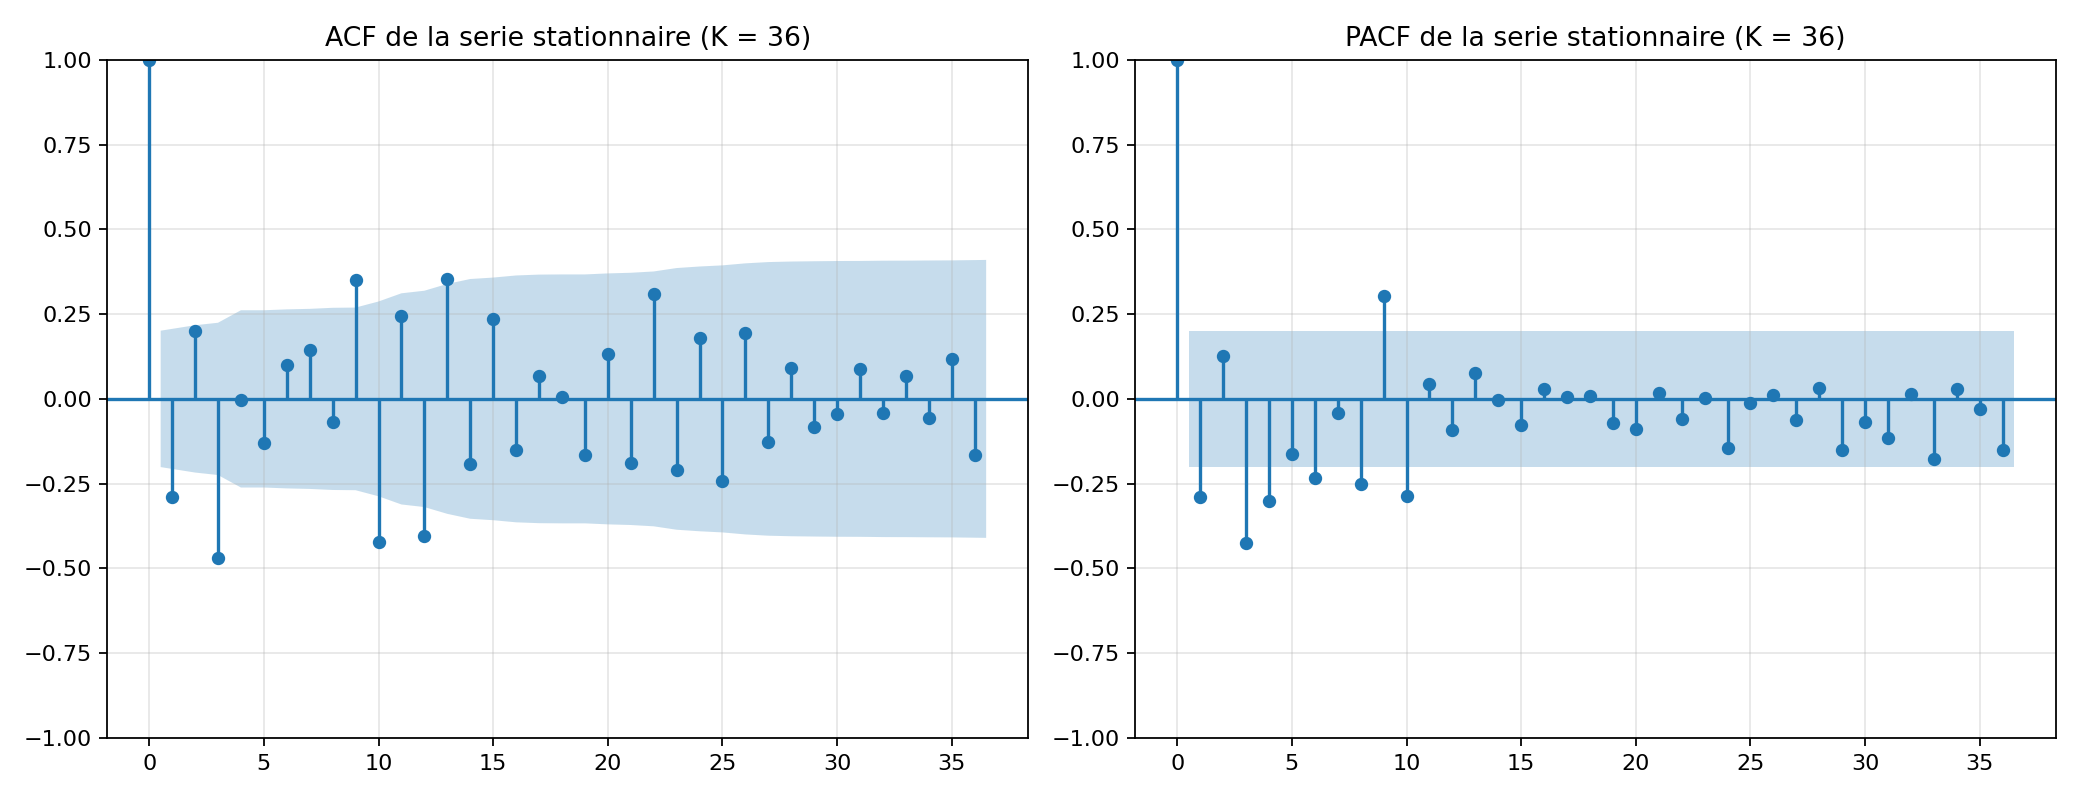
\includegraphics[width=0.92\textwidth]{acf_pacf.png}
\caption{ACF et PACF de la série transformée stationnaire.}
\end{figure}

\section{Modélisation Box-Jenkins}

On estime des modèles SARIMA de la forme :
\[
SARIMA(p,1,q)(P,1,Q)_{12}.
\]
La recherche est volontairement limitée à de petits ordres, afin de garder un modèle
interprétable : $p,q \in \{0,1,2,3\}$ et $P,Q \in \{0,1\}$. Les modèles sont comparés
à l'aide du critère AIC, puis vérifiés par les diagnostics des résidus et par la qualité
de prévision sur l'échantillon de validation.

\begin{table}[H]
\centering
\begin{tabular}{lrrr}
\toprule
Modèle & AIC & BIC & MAPE validation \\
\midrule
SARIMA$(3,1,1)(0,1,0)_{12}$ & -261,25 & -250,15 & 0,73 \% \\
SARIMA$(3,1,2)(0,1,0)_{12}$ & -259,26 & -245,94 & 0,72 \% \\
SARIMA$(0,1,3)(0,1,0)_{12}$ & -256,53 & -247,71 & 4,38 \% \\
SARIMA$(0,1,3)(1,1,0)_{12}$ & -256,29 & -245,90 & 4,76 \% \\
SARIMA$(3,1,3)(0,1,0)_{12}$ & -254,82 & -239,38 & 4,53 \% \\
\bottomrule
\end{tabular}
\caption{Comparaison de quelques modèles candidats.}
\end{table}

Le modèle retenu est donc :
\[
SARIMA(3,1,1)(0,1,0)_{12}.
\]
Sur la série logarithmique, il s'écrit :
\[
(1-\phi_1B-\phi_2B^2-\phi_3B^3)(1-B)(1-B^{12})\log(Y_t)
= (1+\theta_1B)\varepsilon_t.
\]

\section{Validation du modèle}

Les résidus doivent ressembler à un bruit blanc : ils ne doivent pas présenter une
structure temporelle claire. Les diagnostics graphiques sont globalement satisfaisants.
Le test de Ljung-Box à 24 retards donne une p-value de 0,587, ce qui ne permet pas de
rejeter l'hypothèse d'absence d'autocorrélation globale des résidus. Le retard 12 est
légèrement limite, mais le modèle reste très performant en validation et demeure simple
à présenter.

\begin{figure}[H]
\centering
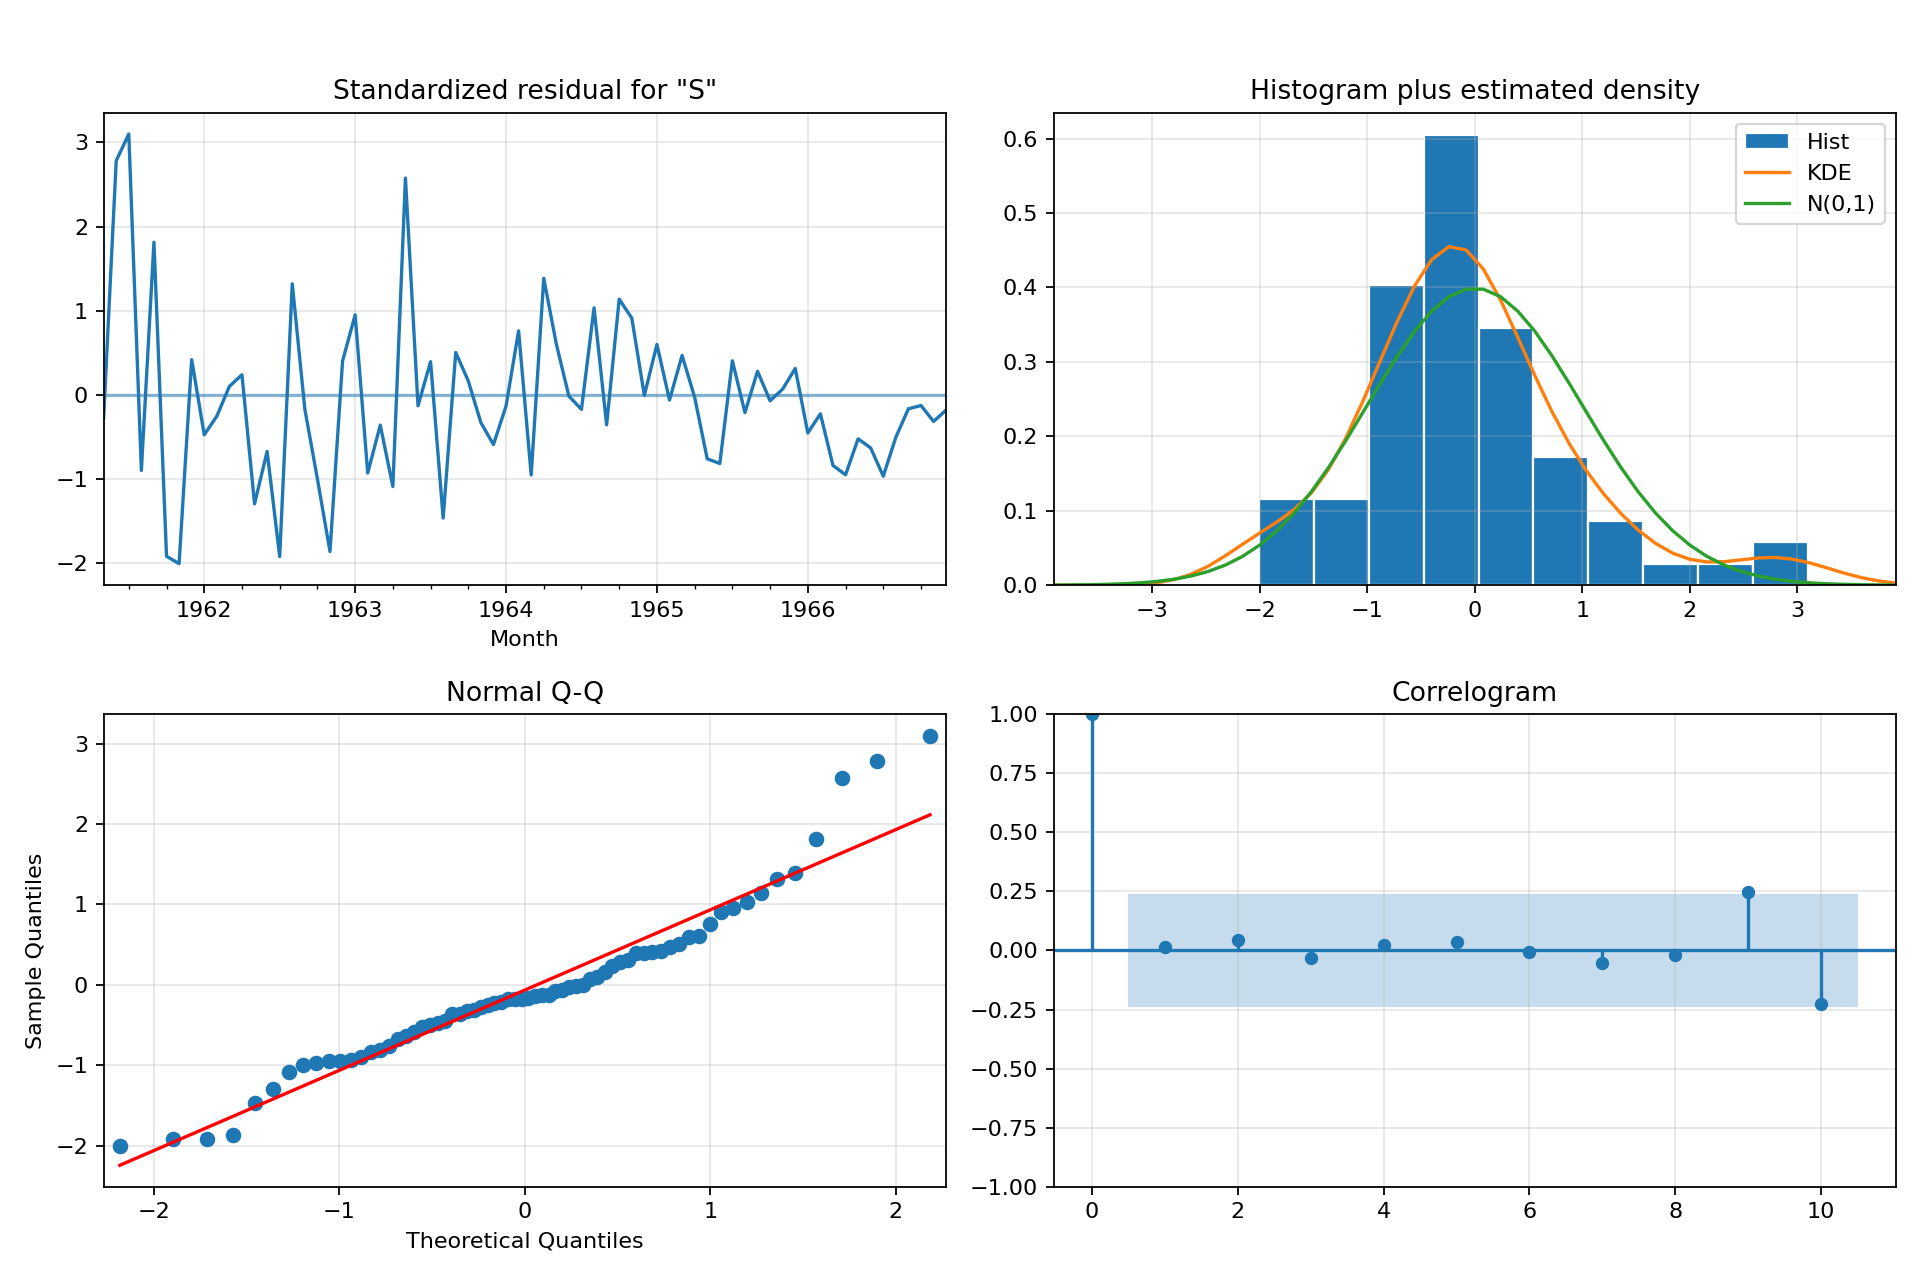
\includegraphics[width=0.92\textwidth]{diagnostics_residus.png}
\caption{Diagnostics des résidus du modèle retenu.}
\end{figure}

\begin{table}[H]
\centering
\begin{tabular}{lr}
\toprule
Indicateur & Valeur \\
\midrule
MAE & 159,99 \\
RMSE & 200,89 \\
MAPE & 0,73 \% \\
\bottomrule
\end{tabular}
\caption{Erreurs de prévision sur l'échantillon de validation.}
\end{table}

Le graphique de validation montre que les prévisions suivent très bien les observations
réelles de 1967 et 1968.

\begin{figure}[H]
\centering
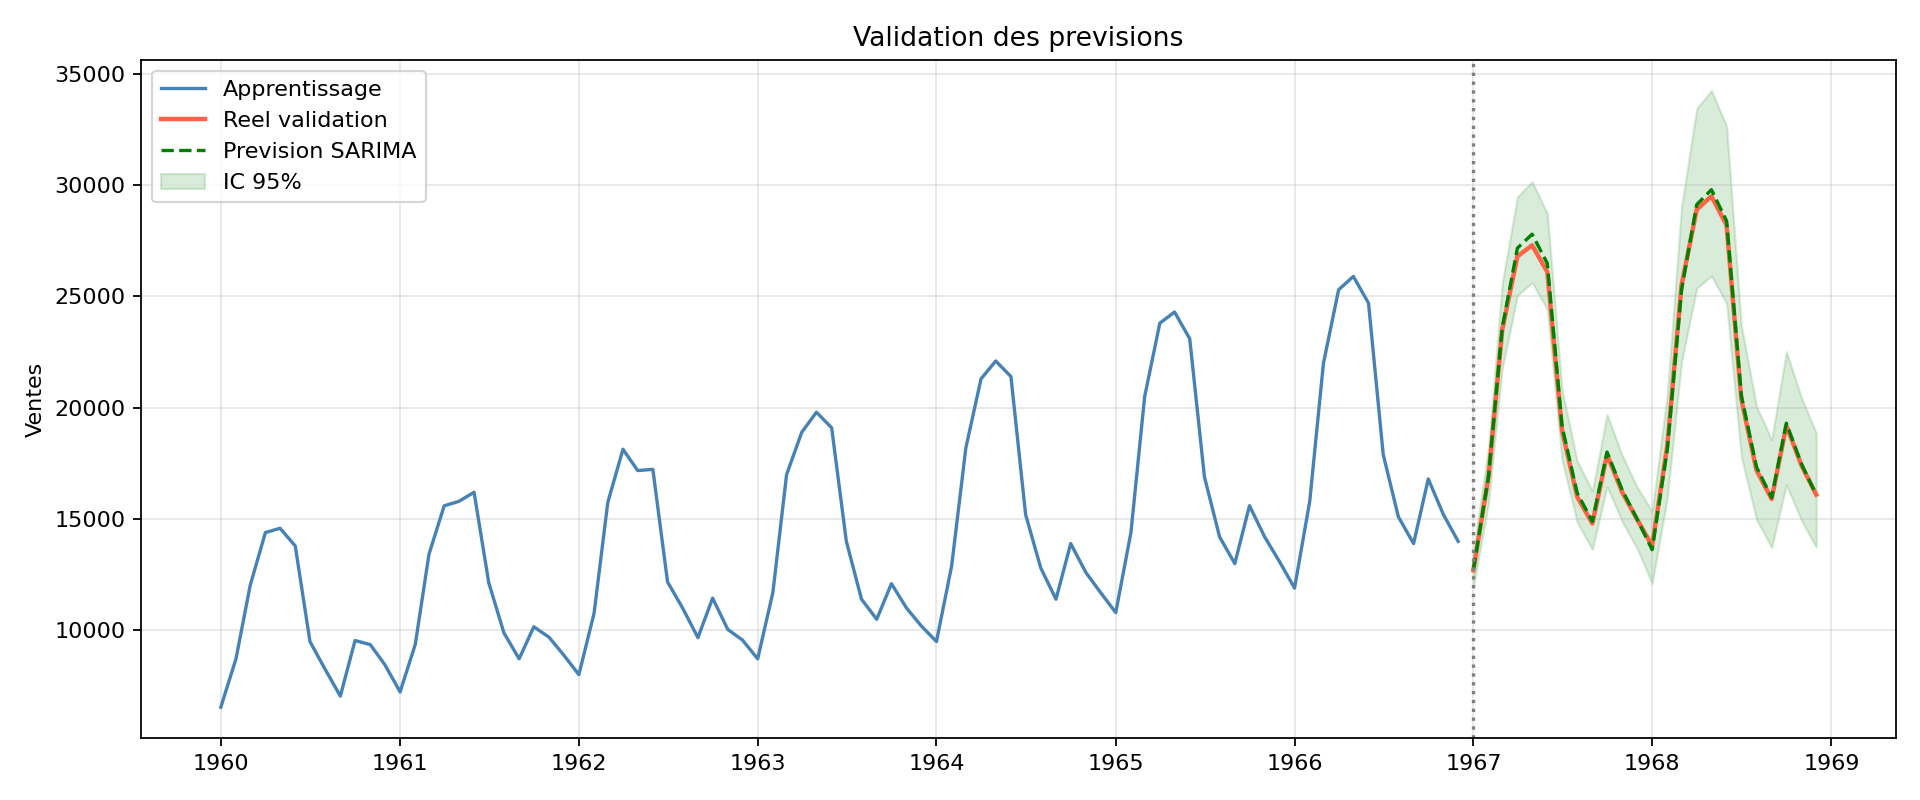
\includegraphics[width=0.92\textwidth]{prevision_validation.png}
\caption{Prévision sur l'échantillon de validation.}
\end{figure}

\section{Prévision finale}

Après validation, le modèle est réestimé sur toute la série disponible, puis utilisé pour
prévoir les ventes mensuelles de l'année 1969.

\begin{figure}[H]
\centering
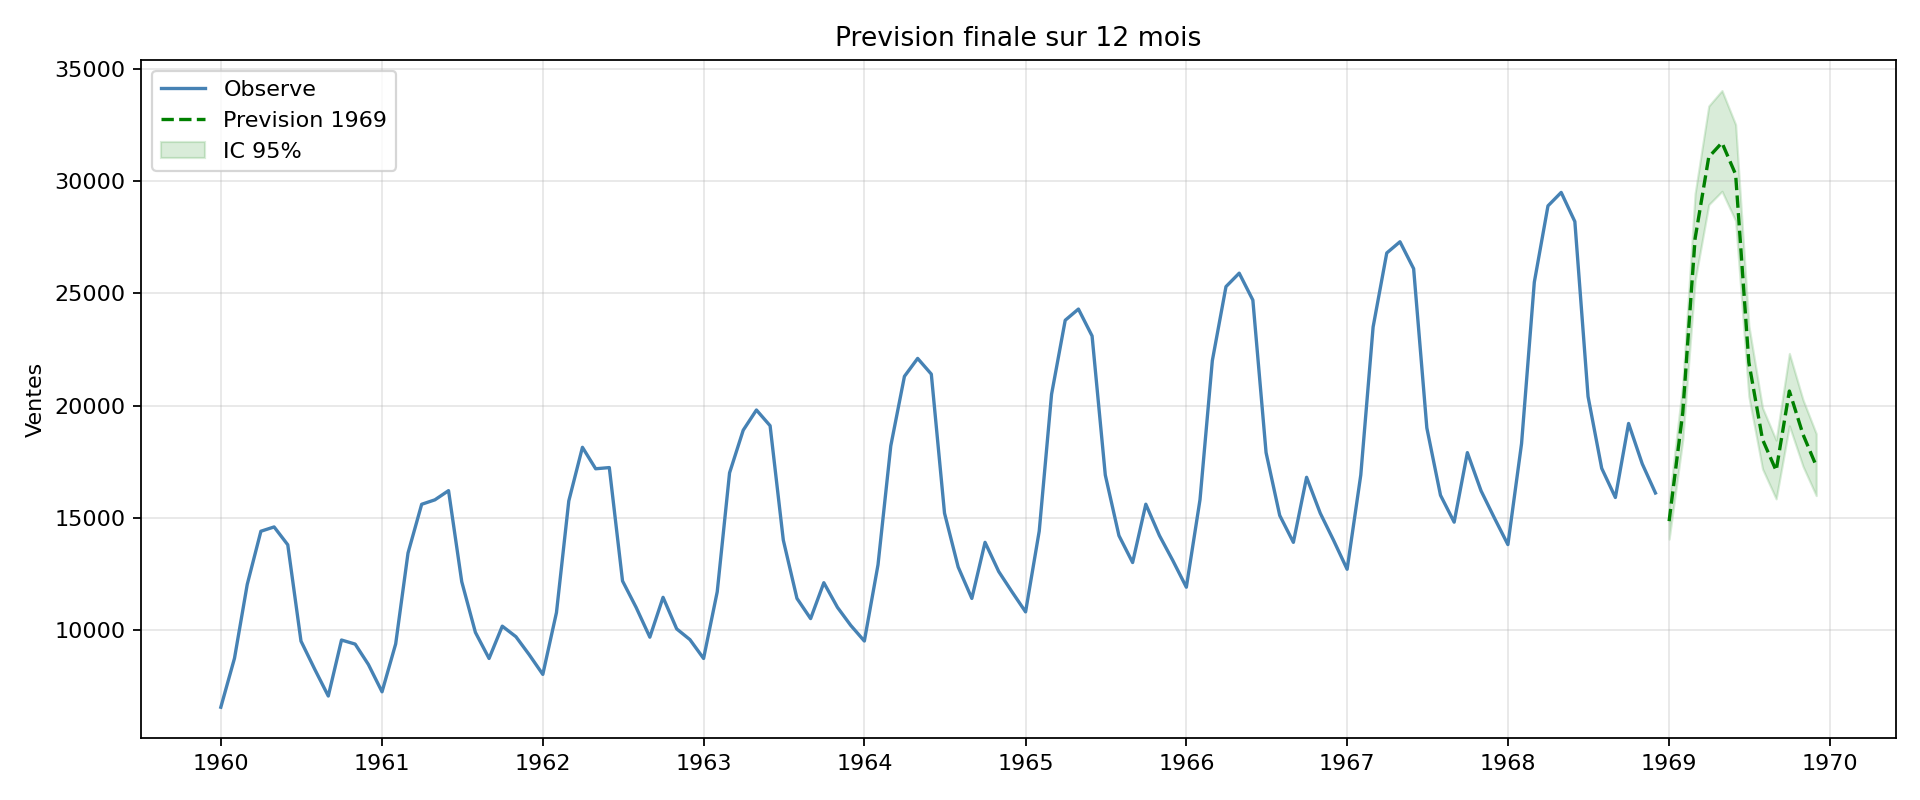
\includegraphics[width=0.92\textwidth]{prevision_1969.png}
\caption{Prévision finale pour l'année 1969.}
\end{figure}

\begin{table}[H]
\centering
\begin{tabular}{lrrr}
\toprule
Mois & Prévision & Borne inf. 95 \% & Borne sup. 95 \% \\
\midrule
1969-01 & 14 844 & 14 043 & 15 691 \\
1969-02 & 19 683 & 18 472 & 20 973 \\
1969-03 & 27 444 & 25 571 & 29 455 \\
1969-04 & 31 076 & 28 954 & 33 352 \\
1969-05 & 31 716 & 29 550 & 34 041 \\
1969-06 & 30 303 & 28 233 & 32 525 \\
1969-07 & 21 927 & 20 406 & 23 562 \\
1969-08 & 18 489 & 17 177 & 19 902 \\
1969-09 & 17 097 & 15 837 & 18 457 \\
1969-10 & 20 645 & 19 094 & 22 323 \\
1969-11 & 18 710 & 17 285 & 20 253 \\
1969-12 & 17 309 & 15 983 & 18 746 \\
\bottomrule
\end{tabular}
\caption{Prévisions finales des ventes pour 1969.}
\end{table}

\section{Conclusion}

La série étudiée présente une tendance croissante et une saisonnalité annuelle nette.
La transformation logarithmique, puis les différenciations ordinaire et saisonnière,
permettent d'obtenir une série stationnaire. La méthode de Box-Jenkins conduit à retenir
un modèle SARIMA$(3,1,1)(0,1,0)_{12}$. Les résultats sur la période de validation sont
très satisfaisants, avec un MAPE inférieur à 1 \%. Les prévisions finales pour 1969
conservent le profil saisonnier observé : niveaux élevés au printemps, puis baisse vers
l'été et l'automne.

Pour une présentation orale, l'idée principale à retenir est simple : la série augmente,
elle est saisonnière, on la stabilise par logarithme et différenciations, puis un modèle
SARIMA permet de prévoir correctement les deux dernières années gardées en validation.

\end{document}
